%\documentclass[iop,twocolumn, tighten, twocolappendix, numberedappendix]{emulateapj}
\documentclass[iop,onecolumn]{revtex4}

\usepackage[backref,breaklinks,colorlinks,citecolor=blue]{hyperref}  
\usepackage[all]{hypcap}
\renewcommand*{\backref}[1]{[#1]}
\newcommand{\x}{\sout}


\usepackage{amsmath}
\usepackage{amssymb}
\usepackage{graphicx}
\usepackage{color}
\usepackage{natbib}
\usepackage{xspace}
\usepackage{nicefrac}
\bibliographystyle{hapj}
\usepackage[dvipsnames]{xcolor}
\newcommand\myshade{85}
\usepackage[T1]{fontenc}
\usepackage{lmodern}
\usepackage{tablefootnote}

 	
\colorlet{mycitecolor}{Turquoise}
\colorlet{mylinkcolor}{Turquoise}

\hypersetup{
 citecolor = mycitecolor!\myshade!black,
 linkcolor = mylinkcolor!\myshade!black,
 colorlinks = true,
}

\def\aj{Astronomical Journal}             % Astronomical Journal
\def\apj{Astrophysical Journal}                % Astrophysical Journal
\def\apjl{Astrophysical Journal}             % Astrophysical Journal, Letters
\def\pasj{PASJ}
\def\apjs{ApJS}              % Astrophysical Journal, Supplement
\def\mnras{MNRAS}            % Monthly Notices of the RAS
\def\prd{Phys.~Rev.~D}       % Physical Review D
\def\prl{Phys.~Rev.~Lett}    % Physical Review Letters
\def\cqg{Class.~Quant.~Grav.~}%Classical and Quantum Gravity
\def\araa{ARA\&A}             % Annual Review of Astron and Astrophys
\def\nat{Nature}              % Nature
\def\aap{A\&A}                % Astronomy and Astrophysics
\def\na{New Astronomy}
\def\nar{New Astronomy Reviews}
\def\pasa{Publications of the Astron.~Soc.~of Australia}
\def\aapr{Astron.~\& Astrophys.~Reviews}
\def\physrep{Physics Reports}


\newcommand{\todo}[1]{\textcolor{red}{#1}}
\newcommand{\tocheck}[1]{\textcolor{green}{Check: #1}}
\newcommand{\citeme}{{\color{magenta} CITE ME!}}

\def\be{\begin{equation}}
\def\ee{\end{equation}}
\def\ba{\begin{eqnarray}}
\def\ea{\end{eqnarray}}
\def\rsquo{'}


%\submitted{Submit ted \today}

\begin{document}

\title{Merging stellar-mass binary black holes}
%\shorttitle{}

\def\addBham{Institute of Gravitational Wave Astronomy and School of Physics and Astronomy, University of Birmingham, Edgbaston, Birmingham B15 2TT, United Kingdom}


\author{Ilya Mandel}
\email{imandel@star.sr.bham.ac.uk}
\affiliation{\addBham}
\author{Alison Farmer}
\affiliation{kW Engineering, Oakland, California, 94612, USA}

\begin{abstract}

LIGO and Virgo detectors has recently directly observed gravitational waves from several pairs of merging stellar-mass black holes, as well as from one neutron star binary.  These observations raise the hope that compact object mergers could be used as a probe of stellar and binary evolution, and perhaps of stellar dynamics.    This informal note summarises the existing observations, describes theoretical predictions for formation channels of merging stellar-mass black-hole binaries along with their rates and observable properties, and presents some of the prospects of gravitational-wave astronomy.

\end{abstract}

\maketitle

\section{Introduction}

The subject of merging stellar-mass binaries as gravitational-wave sources is perfectly suited to an informal colloquium presentation. Several formal reviews were written in the excitement following the first detection \citep{GW150914} of gravitational waves by the Laser Interferometer Gravitational-wave Observatory (LIGO) \citep{GW150914:detectors}, including the astrophysical context companion paper by the the LIGO-Virgo scientific collaboration \citep{GW150914:astro} and the excellent article by \citet{Miller:2016}. More reviews are certainly in the works. However, it is somewhat premature to formally review a field that is both rapidly evolving and very much in its infancy.  With just a few detections to date of gravitational waves from merging black holes \citep{GW150914,GW151226,BBH:O1,GW170104,GW170608,GW170814}, and one from merging neutron stars \citep{GW170817}, we are only beginning to explore the population of merging compact-object binaries.  We are not yet certain of the dominant formation channels for these sources, or even of the full range of astrophysical questions that gravitational-wave observations will answer. It is clear, however, that there are many important and exciting questions to explore.

\textcolor{red}{Can we go bigger picture here and say (briefly) why binary star evolution is interesting and/or important? A very quick summary of the Prospects section?}

In this colloquium paper, we focus on the questions that strike us as being most interesting and timely at this stage of the field's development.  These will indeed mostly be questions rather than answers, and the list is undoubtedly biased by our own interests. Further, we do not attempt to systematically survey all of the relevant literature.  In other words, this is emphatically {\it not} a review. \textcolor{red}{Can we summarize the questions in one or two sentences? Understanding the evolution of massive stellar binaries? Something else?}


Below, we summarise the existing observations of merging binary black holes and closely related systems in section \ref{obs}, describe the plausible formation scenarios for binary black holes in \autoref{form}, discuss the predicted merger rates and merging object properties in \autoref{merge}, and speculate about the prospects for gravitational-wave astronomy in \autoref{prospect}.


 

\section{Observations}\label{obs}

\subsection{Gravitational-wave observations}


\subsubsection{The confirmed detections to date}
During its first science run, lasting from September of 2015 through January of 2016, the LIGO detector network observed three likely signals from the mergers of binary black holes.  GW150914 \citep{GW150914} and GW151226 \citep{GW151226} were confident, $> 5\sigma$ observations; LVT151012 was estimated as having a $\sim 90\%$ probability of being a gravitational-wave signal \citep{GW150914:rates,BBH:O1}, though the estimate is conservative and we shall treat it as a detection here.  During the second science run, lasting with some interruptions from November 2016 through August 2017, three further confident binary black hole detections have been announced: GW170104 \citep{GW170104},  GW170608 \citep{GW170608}, and GW170814 \citep{GW170814}, the last of them with the participation of the Virgo gravitational-wave observatory.   The observation of gravitational waves from the binary neutron star merger GW170817 \citep{GW170817} was followed up by an unprecedented campaign of electromagnetic observations, leading to detections of a short gamma ray burst, optical kilonova, and an afterglow spanning from radio through X-ray wavelengths \citep{GW170817:GRB,GW170817:MMA}.  We shall focus on binary black holes here.

\subsubsection{Information encoded in GW signals}
The gravitational-wave signature of a merging binary encodes the properties of the binary: the component masses and spins. Coupled with information from two or more detectors in a network, this makes it possible to infer the sky location and orientation of the source and the distance to the source \citep{Veitch:2015,GW150914:PE}.  However, some of the source parameters are strongly correlated, leading to near-degeneracies when attempting to extract them from a noisy data set.   For the heaviest black hole binaries such as GW150914, the total mass $M \equiv M_1 + M_2$ is measured relatively accurately as the ringdown, whose frequency is a function of the total mass, falls in the sensitive frequency band of the gravitational-wave detectors.  For most black holes, the chirp mass $M_c \equiv M_1^{3/5} M_2^{3/5} M^{-1/5}$ is the better measured parameter, since it determines to lowest order the rate of the frequency evolution during the inspiral phase.  The mass ratio $q\equiv M_2/M_1 \leq 1$ is often quite poorly constrained, because it enters the inspiral phasing at a higher order in the ratio of the orbital velocity to the speed of light and is partially degenerate with the black hole spins \citep[e.g.,][]{PoissonWill:1995}.  

\subsubsection{Information extracted from the observed GW signals}
We list the parameters of the black holes observed to date in table \ref{table:BHmasses}. Specific system properties are discussed below.

\textbf{Mass Ratios:} While all binary black holes observed today are consistent with having equal-mass components, mass ratios could be as extreme as $4:1$ in some cases.  

 
\begin{table}
\begin{tabular}{lcccccc}
Event  & $M_c$ [$M_\odot$]  & q & $M_1$ [$M_\odot$]  & $M_2$ [$M_\odot$]  & $\chi_\textrm{eff}$ & $d_L$ [Mpc] \\
\hline
GW150914\footnote{\citet{BBH:O1}} & $28.1^{+1.8}_{-1.5}$ & $0.81^{+0.17}_{-0.2}$ & $36.2^{+5.2}_{-3.8}$ & $29.1^{+3.7}_{-4.4}$ & $-0.06^{+0.14}_{-0.14}$ & $420^{+150}_{-180}$\\
LVT151012$^\mathrm{a}$ & $15.1^{+1.4}_{-1.1}$ &$0.57^{+0.38}_{-0.37}$ &$23^{+18}_{-6}$ &$13^{+4}_{-5}$ &$0.03^{+0.31}_{-0.20}$ &$1020^{+500}_{-490}$\\
GW151226$^\mathrm{a}$ & $8.88^{+0.33}_{-0.28}$ &$0.52^{+0.40}_{-0.29}$ &$14.2^{+8.3}_{-3.7}$ &$7.5^{+2.3}_{-2.3}$ &$0.21^{+0.20}_{-0.10}$ &$440^{+180}_{-190}$ \\
GW170104\footnote{\citet{GW170104}} & $25.1^{+2.5}_{-3.9}$ &$0.62^{+0.32}_{-0.26}$ &$31.2^{+8.4}_{-6.0}$ &$19.4^{+5.3}_{-5.9}$ &$-0.12^{+0.21}_{-0.30}$ &$880^{+450}_{-390}$\\
GW170608\footnote{\citet{GW170608}} & $7.9^{+0.2}_{-0.2}$ &$0.6^{+0.3}_{-0.4}$ &$12^{+7}_{-2}$ &$7^{+2}_{-2}$ &$0.07^{+0.23}_{-0.09}$ &$340^{+140}_{-140}$ \\
GW170814\footnote{\citet{GW170814}} & $24.1^{+1.4}_{-1.1}$ & &$30.5^{+5.7}_{-3.0}$ &$25.3^{+2.8}_{-4.2}$ &$0.06^{+0.12}_{-0.12}$ & $540^{+130}_{-210}$ \\
\hline
\end{tabular}
\caption{The inferred parameters of the merging binary black holes.  The median value and the 90\% credible interval bounds are given.}\label{table:BHmasses}
\end{table}


%GW150914 has the heaviest black holes, allowing the total mass $M \equiv M_1 + M_2$ to be particularly well measured as the merger and ringdown fall in the sensitive frequency band of the detectors: $65 \pm 4\, M_\odot$ in the source frame.  For the other two events with lighter black holes, the chirp mass $M_c \equiv M_1^{3/5} M_2^{3/5} M^{-1/5}$ is the better measured parameter; $M_c = 15 \pm 1\, M_\odot$ for LVT151012 and  $M_c = 8.9 \pm 0.3\, M_\odot$ for GW151226.  The mass ratio is relatively well constrained toward equal masses for GW150914, providing confidence that both components weigh in within a few solar masses of $30\, M_\odot$.  On the other hand, while LVT151012 and GW151226 may be signals from mergers of nearly equal-mass $\sim 17\, M_\odot$ and $\sim 10\, M_\odot$ black holes, respectively, the black hole masses could also be very unequal for these events, as the mass ratios could be as extreme as $4:1$ and $3:1$, respectively. 

%\todo {Add newest detections.  Table?  Better yet, figure, including XRBs and uncertainties?}

\textbf{Black Hole Spins:} Individual black hole spins are difficult to measure precisely with gravitational waves.  However, we do know that none of the observed binaries could have large spins aligned with the orbital angular momentum; in fact the averaged dimensionless spin along the direction of the orbital angular momentum $\chi_\textrm{eff}$ is below $0.4$ for all observed events, and consistent with zero for all but one of them.  Interestingly, it is not consistent with zero for GW151226, the second lightest binary black hole detected, indicating that at least one of the components for that event must have been a rotating Kerr black hole.  Spin projections in the orbital plane are very poorly constrained for all events.

\textbf{Distances:} All signals came from distances of around 500 Mpc to 1 Gpc (redshifts $z\sim 0.1$ -- $0.2$).  With just two operational detectors, LIGO Hanford and LIGO Livingston, for all events prior to GW170814, sources could only be localised to 90\% credible regions spanning hundreds to more than a thousand square degrees on the sky.  The participation of the Virgo instrument in the observation of GW170608 reduced the sky region to only 60 deg$^2$.  Nonetheless, associations with specific host galaxies are impossible for all binary black hole mergers.  

\textbf{Mass Distribution:} Sensitivity to gravitational waves from binary mergers depends on the object mass; the horizon distance at which a source is detectable scales as $M_c^{5/6}$ for inspiral-dominated signals, so the surveyed volume scales as $M_c^{2.5}$.  While three observations are not sufficient to determine the mass distribution of merging binary black holes, the observed broad mass distribution, deconvolved with the mass-dependent selection effects, could be consistent with an intrinsic mass distribution of $M^{-2.5}$, reminiscent of the stellar initial mass function \citep{Salpeter:1955}.  The uncertainty in the mass distribution is relayed into the uncertainty on inferred merger rates; these later are consistent with a broad range spanning $\sim 10$ -- $200$ Gpc$^{-3}$ yr$^{-1}$.  
%mass distribution is a more derived quantity than any of the others mentioned above. Is there a better place for this?

\textbf{Testing General Relativity:} All LIGO signals observed to date are consistent with gravitational waves expected within the general theory of relativity, providing a stringent test of this theory in the dynamical, strong-field regime \citep{GW150914:GR}.

\subsection{Electromagnetic observations}
%This section is currently very jargony... lots of terms that will mystify the non-astro student.

\subsubsection{Electromagnetic observations as complementary probes}

\textcolor{red}{Placeholder intro paragraph -- this section needs an intro.} The systems that eventually become merging binary black holes have most likely passed through a number of other phases of existence, including phases in which the system or its component stars emitted electromagnetic radiation. Many other binary evolution pathways are possible, including a large fraction which do not end as a binary black hole merger. Binary evolutionary pathways are discussed in more detail in \autoref{form}. In this section we describe some of the key electromagnetic observations that -- together with the GW observations of merging black holes -- shed light on the evolution of massive stellar binaries.

Many electromagnetic observations of binary stars have been made over the years. \textcolor{red}{Want to make it clear here that the more mature field is the EM one, but that GWs have suddenly invigorated things?} A subset of these shed light on various intermediate stages of compact object binary formation and evolution preceding merger. These include observations of initial mass and period distributions of massive stellar binaries \citep[e.g.,][]{Sana:2012}, and observations of luminous red novae, which may be associated with common envelope events \citep{Ivanova:2013LRN}. These also include observations of supernovae, X-ray binaries (including Be X-ray binaries, and ultra-luminous X-ray binaries -- and other types??), Galactic binary radio pulsars, and gamma ray bursts. We focus here on black hole X-ray binaries, the type of binary star with the closest connection to merging binary black holes.

%observations of mass and period distributions of luminous red novae or just observations of them in general??

\subsubsection{X-Ray Binaries}

\textcolor{red}{Say (briefly) what an X-ray binary is?} We focus here on observations of X-ray binaries containing a black hole accreting mass from a companion, either through wind-driven mass loss and Bondi-Hoyle accretion (high-mass X-ray binaries) or Roche lobe overflow from a companion that has expanded beyond the $L_1$ Lagrange point  (low-mass X-ray binaries).   \textcolor{red}{jargooooon}
Some of the observed high-mass X-ray binaries may ultimately produce gravitational-wave sources \citep{CygnusX3:2012}.  %what do you mean by "ultimately produce GW sources?"

\textbf{Black hole masses:} 
 Black-hole X-ray binaries with dynamical mass measurements provide the only other secure measurements of black hole masses in addition to the gravitational-wave observations described above.  \citet{Ozel:2010} and \citet{Farr:2011} summarize the mass distribution of black-hole X-ray binaries; they find a distribution which ranges from 4 or 5 solar masses on the low-mass end (with a possible mass gap between neutron star and black hole masses) to $\sim 15\, M_\odot$ or more on the high mass end.  However, given the doubts subsequently placed on the radial velocity measurements in high-mass X-ray binaries such as IC10 X-1 \citep{Laycock:2015}, there are no known black holes with dynamically confirmed masses guaranteed to exceed $15\, M_\odot$.  The masses of black holes in X-ray binaries are sketched in figure \ref{fig:BHmasses} along with the masses of gravitational-wave sources.  This figure does not include speculative but potentially very exciting intermediate-mass black holes \citep{MillerColbert:2004,Pasham:2014}; if such few-hundred solar-mass black holes generically exist in globular clusters, they will be detectable as gravitational-wave sources \citep[e.g.,][]{Mandel:2008}.
%\todo{Add GC X-ray binary observations} 

\begin{figure}
	\centering
	%\includegraphics[trim={1.3cm 7.0cm 0.0cm 7.9cm},clip,scale=0.45]{evolvedPvseWithOrbit.pdf}
	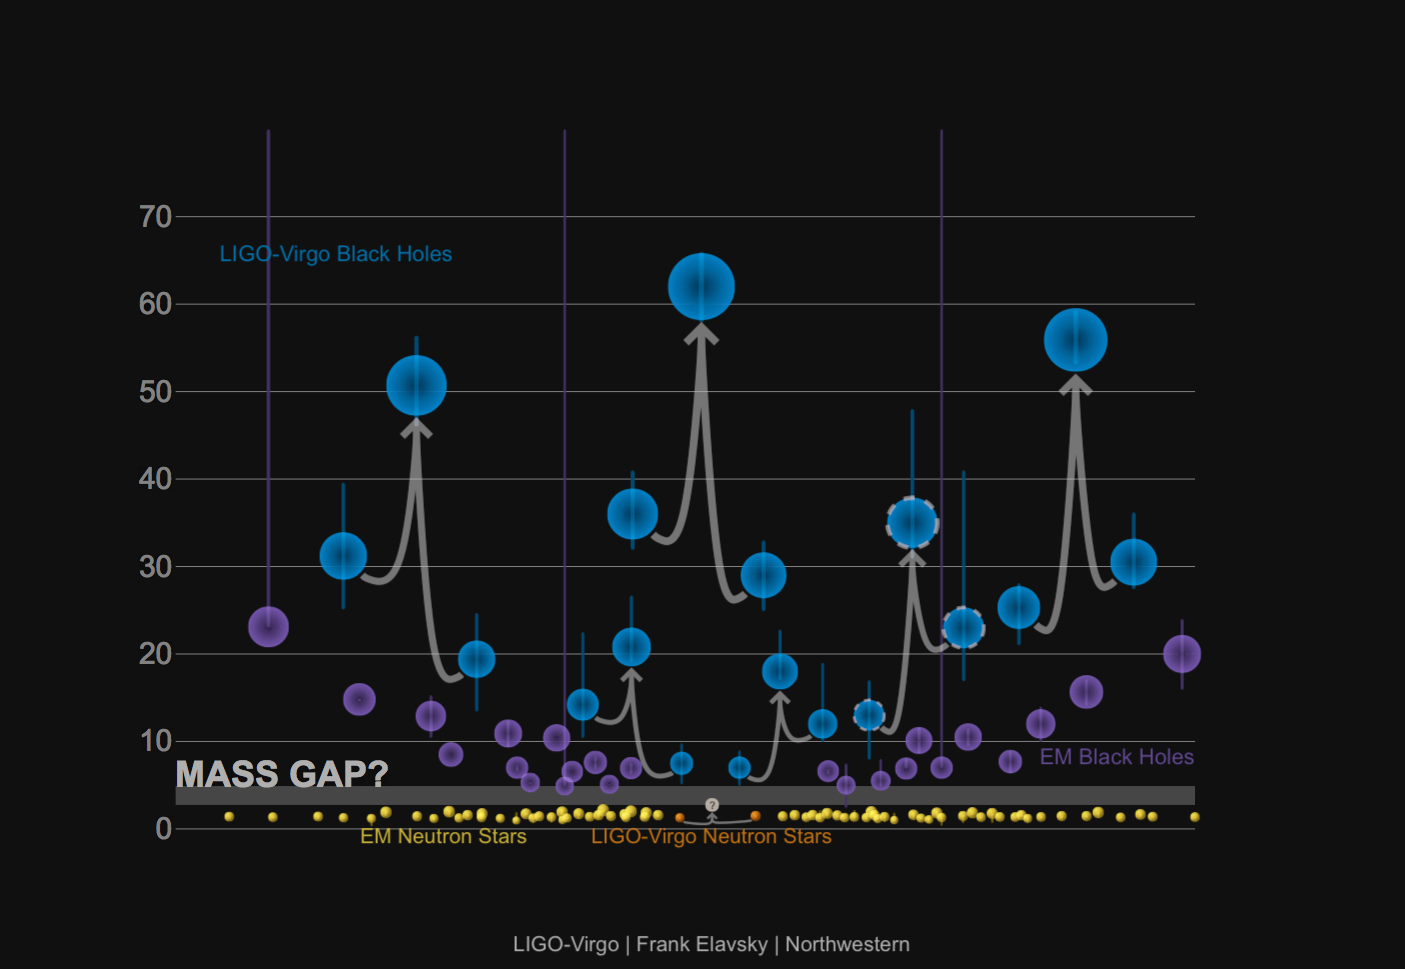
\includegraphics[width=0.99\textwidth]{Graveyard-linear.png}%{BHmass.png}
	\caption{\label{fig:BHmasses}  The masses (in solar masses, vertical axis) of black holes observed as gravitational-wave sources (blue), as well as masses of black holes in X-ray binaries (purple).  Galactic neutron stars observed as radio pulsars (yellow) and the merging double neutron star GW170817 (orange) appear at the bottom of the figure.  Placement on the horizontal axis is arbitrary.  Error bars are indicative of the measurement uncertainty.  Figure courtesy of Frank Elavsky, Northwestern University and LIGO-Virgo collaborations.}
\end{figure}


\textbf{Black Hole Spin Magnitudes:} Black hole X-ray binaries also provide an opportunity for measuring black hole spins \citep[see][for a recent review]{MillerMiller:2015}.  Continuum fitting of the X-ray flux from the disk and iron K-$\alpha$ line fits to the disk reflection profile can both be used to infer the location of the inner edge of the disk, assumed to correspond to the radius of the innermost stable circular orbit, which is a sensitive function of black hole spin.  Quasi-periodic oscillations also have the potential to provide spin measurements.  Unfortunately, the underlying physical mechanisms are not fully understood at present, and the models can suffer from significant systematics.  For example, for 2 of 6 systems for which both disk continuum and disk reflection spin measurements are available, the two methods are inconsistent at the $3$ or $5$ sigma level, and for one system the statistical uncertainty is so large as to span nearly the full allowed range from $0$ to $1$.  However, for the remaining 3 systems with both measurements available, both methods yield spins $\chi \gtrsim 0.9$.  

\textbf{Inconsistency with Spin Observations from GW Sources?} Most relevantly, these high-spin observations include two high-mass X-ray binaries: LMC X-1 and Cygnus X-1.  This is significant, because unlike long-lived low-mass X-ray binaries, whose spin magnitudes could be altered by accretion from the companion, especially if they started out with intermediate-mass companions \citep{Podsiadlowski:2003,Fragos:2015}, high-mass X-ray binaries are too short-lived to enable significant spin changes due to accretion \citep{KingKolb:1999}.  %Moreover, such high-mass X-ray binaries may be direct progenitors of merging binary black holes \citep{Bulik:2008,CygnusX3:2012}; in fact, 
Isolated binaries that form binary black holes must go through the high-mass X-ray binary phase during their evolution.  Thus, if the high spin magnitude measurements in black-hole X-ray binaries are to be believed, at least some stellar-mass black holes in systems similar to those that could go on to become merging black holes should have high spins; however, there may be significant differences in the evolutionary channels and environments of the locally observed high-mass X-ray binaries and the LIGO-observed binary black holes \citep{HotokezakaPiran:2017}.  Moreover, the spin magnitude measurements could be very sensitive to the modelling assumptions, and the systematic errors may dominated the claimed statistical ones \citep[e.g.,][]{Basak:2017,Kawano:2017}.

\textbf{Black Hole Spin Directions:} We know even less about the spin directions than the spin magnitudes.  Although black-hole spin-orbit alignment is assumed in continuum flux measurements \citep{MillerMiller:2015}, some black-hole X-ray binaries, including GRO J1655-40 \citep{Martin:2008}, 4U 1543-47 \citep{MorningstarMiller:2014} and particularly V4641 Sgr \citep{Orosz:2001,Martin:2008b} appear to indicate that the micro
quasar jet, presumably aligned with the BH spin axis, is misaligned with the orbit.  Moreover, initial stellar spins in massive binaries have been observed to be misaligned \citep[e.g.,][]{Albrecht:2009,Albrecht:2014}, though there are opportunities for realignment during binary evolution, as described below.

\section{Formation scenarios}\label{form}

\textcolor{red}{Section needs an intro.}

When the detection of GW150914 was first announced, many were surprised that it was a binary black hole rather than a binary neutron star \textcolor{red}{(Need to say why people were surprised by BHs not NSs.)} -- and even more surprised by the high black hole masses, in excess of the observed black hole masses in X-ray binaries.  Should this be a source of surprise? 
The short answer is that the masses themselves should not be surprising -- but perhaps the very existence of merging neutron stars and black holes should be.  But let us start with the masses.  

\subsubsection{Understanding the masses of the merging black holes}

\textcolor{red}{Needs intro summary sentence. Placeholder: The apparent discrepancy between BH masses in GW mergers and those in observed X-ray binaries can be understood in terms of the chemical composition of the stars that formed them.}

Compact object masses in double compact object binaries are set by the mass of the star before the collapse or supernova explosion at the end of stellar evolution and the physics of the collapse itself.  The compact object is unlikely to accrete a significant amount of mass after collapse: doubling its mass at the Eddington limit, which corresponds to an equilibrium between the pressure of radiation released during accretion on the infalling material and gravity, would take more than 100 million years, and the massive companion will only survive for a small fraction of that time.  The mass of the compact remnant is thus set by the pre-collapse mass of the stellar core: the convective region in the center of the star where nuclear fusion proceeds from hydrogen through helium, carbon, oxygen, and so on up through iron.  Observational evidence and collapse models suggest that sufficiently massive stellar cores may completely collapse into black holes \citep[for a review, see][]{Mirabel:2016}.  Thus, the mass of the stellar core determines the ultimate black hole mass.  If left unperturbed, perhaps a third of the mass of a heavy star will end up in a carbon--oxygen core.  Since stars well in excess of 100 $M_\odot$ have been observed in the local Universe \citep[e.g.,][]{Schneider:2018}, perhaps the right question to ask is not why LIGO observed such heavy black holes, but why we haven't observed such heavy black holes before?  

The answer has to do with the mass loss from massive stars.  The intense radiation from these stars -- they may have luminosities of order a hundred thousand times greater than the Sun -- drives significant winds, which can remove much of the material from the star.  Metals like iron, with their many absorption lines, are particularly efficient at capturing the radiation and transforming it into outward momentum.  Therefore, the metal fraction, or metallicity, is a key ingredient in determining stellar winds \citep{Vink:2001}.  Although wind models are uncertain \citep[e.g.,][]{Renzo:2017}, simulations suggest that at the metallicity of our solar neighborhood (where roughly 2\% of the stellar matter by mass are metals -- elements heavier than hydrogen and helium, formed by earlier stellar generations rather than during the Big Bang), the maximum black hole masses are only around $15 M_\odot$ \citep{Belczynski:2009,Spera:2015}.  This matches the observations described in the previous section.  Thus, forming heavier black holes requires stellar progenitors born in regions with lower metallicity, that is, fewer preceding stellar generations.  This might either involve low-mass metal-poor galaxies, or formation in the very distant past with a long delay time between star formation and the relatively local black hole mergers \citep{Belczynski:2016}, but more on that below.  Figure \ref{fig:BHremnant} illustrates this by showing the compact remnant (neutron star or black hole) mass as a function of the zero-age main sequence stellar mass as modeled with the COMPAS binary population synthesis code (see \url{http://www.sr.bham.ac.uk/compas}).

\begin{figure}
	\centering
	%\includegraphics[trim={1.3cm 7.0cm 0.0cm 7.9cm},clip,scale=0.45]{evolvedPvseWithOrbit.pdf}
	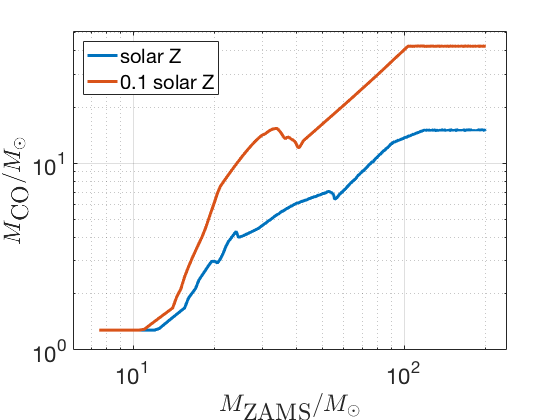
\includegraphics[width=0.7\textwidth]{BHremnantdelayed.png}
	\caption{\label{fig:BHremnant} Remnant compact object mass for a given zero-age main sequence stellar mass in the absence of an interacting binary companion, following the default COMPAS prescription for winds \citep{Stevenson:2017}  and the `delayed' supernova fallback prescription \citep{Fryer:2012}, at solar ($Z_\odot=0.02$) metallicity (blue) and a tenth solar (red).}
\end{figure}
%\todo{Include mass plots from Ben, or reuse Chris's old plot?, or attached?}

\subsubsection{The Separation Question}
The more surprising question, and perhaps the key problem of gravitational-wave astronomy, is why compact object binaries ever merge at all.  And this one boils down to separation.  

Gravitational-wave emission is a very strong function of separation.  Gravitational waves can certainly remove a lot of energy very quickly: the peak gravitational-wave luminosity during a compact binary merger is a few thousandth of the Planck luminosity, $c^5/G$ \citep[e.g.,][]{Cardoso:2018}; at nearly $10^{57}$ erg per second, such mergers 'outshine' all the stars in the visible Universe combined.  But gravitational-wave luminosity is inversely proportional to the fifth power of the binary separation \citep{Peters:1964}, so widely separated binaries lose energy and inspiral very slowly.  \autoref{fig:periapsis} shows the maximum periapsis separation that a binary composed of two equal-mass compact objects can have and still merge within the age of the Universe.  Thirty-solar mass double black holes such as those responsible for GW150914 would have had to start with a separation of less than 50 solar radii, or a quarter of the distance from the Earth to the Sun, if they were to be driven to merger by gravitational-wave emission alone.

On the other hand, massive stars expand.  Even our Sun will reach the size of an astronomical unit during its giant phase; the more massive stars that make neutron stars (around 8 to 20 solar masses at birth) and black holes (above 20 solar masses at birth) may reach sizes of thousands of solar radii at their maximal extent, as shown in \autoref{fig:Rmax}.  Thus, we appear to have an insurmountable problem.  If the stars start out at the separations where gravitational waves could bring their remnants together, the stars will exceed this separation during their evolution and merge long before they collapse into compact objects. If they start sufficiently far apart to avoid this merger while they are still stars, they would require millions of times longer than the age of the Universe to merge, so we could never detect such mergers.  The problem is even worse for double neutron stars than double black holes: because the merger timescale is inversely proportional to the cube of the masses, the double neutron stars must be separated by less than 5 solar radii to merge in the age of the Universe, meaning that, even at birth, their progenitor stars could not fit into a binary of this size.  Thus, we are not so much fitting a square peg into a round hole as fitting a peg into a hole that is around a hundred times too small for the peg!

\begin{figure}
	\centering
	%\includegraphics[trim={1.3cm 7.0cm 0.0cm 7.9cm},clip,scale=0.45]{evolvedPvseWithOrbit.pdf}
	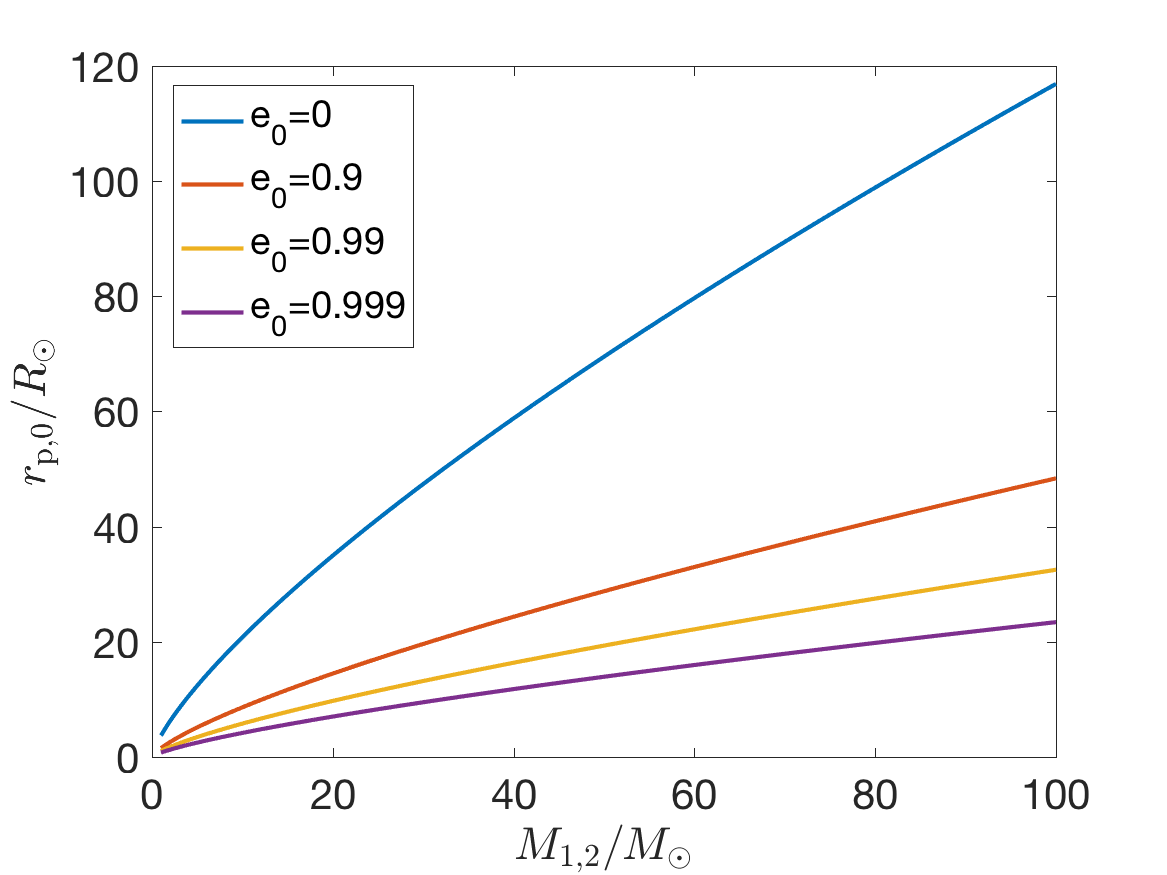
\includegraphics[width=0.45\textwidth]{M-rp.png}
	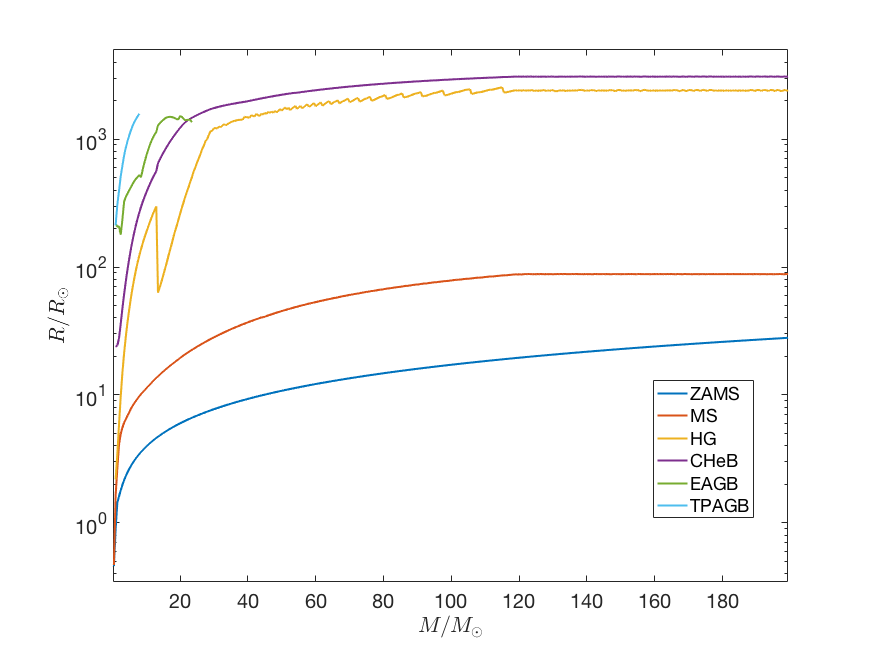
\includegraphics[width=0.45\textwidth]{StellarRadiusZsolar.png}
	\caption{Maximum initial periapsis separation that a binary black hole with equal-mass components (as given on the ordinate) can have to merge in the age of the Universe through gravitational-wave emission.	\label{fig:periapsis}  Right panel: maximal stellar extent at solar metallicity during various phases of stellar evolution for a non-rotating star with a given initial mass; based on the COMPAS implementation of single stellar evolution models of \citet{Hurley:2000}. \label{fig:Rmax} Progenitors of binary black holes grow too large to fit into a binary that would merge through gravitational-wave radiation reaction without engaging in mass transfer first.}
\end{figure}

%\todo{Update left panel of plot to show periapsis on horizontal axis.  Take max radial extent plot from Simon?}

So, how can we overcome this problem of separations, which one grandly label the Fundamental Problem of Gravitational-wave Astrophysics?  After a bit of thought, three possibilities come to mind: (i) fine-tune binary evolution so that the two stars are brought closer together after they have expanded; (ii) wave a magic want and chant ``Abracadabra! Stars, thou shalt not expand!''; (iii) let the stars expand and form black holes in isolation, and only bring them together after they have done so.  Crazy as these may sound, they all might plausibly contribute to the formation of binary black holes, as we discuss below.  [We won't discuss the proposed fragmentation of a single stellar core into two black holes \citep{Loeb:2016} -- \citet{Woosley:2016,Dai:2017} discuss the problems with this picture -- or non-astrophysical formation scenarios such as primordial black holes of cosmological origin \citep[e.g.,][]{Bird:2016}.]

\subsection{Bring the stars together after they have expanded: classical isolated binary evolution via the common-envelope phase}

The first possible channel is perhaps the most studied one, with the first mention coming as early as \citet{Tutukov:1973}.  In this channel, the two stars are born in a relatively wide binary, allowing them space to expand.  However, at a critical moment, the binary is hardened by a factor of two or more orders of magnitude through dynamically unstable mass transfer, known as a common envelope phase, allowing the compact object binary to ultimately merge through gravitational-wave emission.  This channel has been studied at length over the past 40 years, with significant contributions coming from \citet{TutukovYungelson:1993,Lipunov:1997,BetheBrown:1998,Nelemans:2003,VossTauris:2003,Pfahl:2005,Dewi:2006,Kalogera:2007,OShaughnessy:2008,Dominik:2012,Dominik:2014, Belczynski:2016,EldridgeStanway:2016} and many others.  Rather than summarizing all of the steps and challenges in massive binary evolution (see the papers above and the review by \citet{PostnovYungelson:2014} for details), we will illustrate the possible formation of a binary using a simulation from the COMPAS binary population synthesis code \citep{Stevenson:2017} that leads to the formation of a GW150914-like merging system.

The evolution of this system is sketched out in an van den Heuvel -- style diagram in \autoref{fig:COMPAS}.  Two massive stars of perhaps $100$ and $75$ solar masses are born in a low-metallicity environment ($\sim 5\%$ of solar metallicity)  binary at a separation of $\sim 10$ AU.  The more massive primary reaches the end of its main sequence first.  At this stage, it has completed fusing hydrogen into helium in the core, and with the loss of energy input, the core begins to contract.  The release of gravitational binding energy and the onset of hydrogen shell burning cause the hydrogen-rich envelope to expand, until the primary expands past the L1 point and overflows its Roche Lobe, beginning to transfer mass onto the secondary.  The mass transfer proceeds on the thermal timescale of the primary donor and is likely significantly non-conservative, as the less evolved secondary, with its correspondingly longer thermal timescale, is unable to accept mass at the rate it is being donated.  The loss of mass from the binary further widens the system, to perhaps $\sim 20$ AU.  The primary loses its entire envelope, leaving behind a naked helium-burning star -- a Wolf-Rayet star.  Following wind-driven mass loss, which further widens the system, the primary collapses into a black hole; here, this collapse is assumed to be complete, without an associated natal kick.  When, a few hundred thousand years later, the secondary reaches the end of its main sequence, the process repeats in reverse: the secondary expands until it commences mass transfer onto the primary.  By this time, the primary has lost around two thirds of its initial mass through a combination of envelope stripping, winds, and possible mass loss during a supernova.  Meanwhile, this mass transfer would need to be almost wholly non-conservative if the accretion onto the black hole obeys the Eddington limit.  Consequently, mass transfer would lead to a rapid hardening of the binary at a rate that is faster than the reduction in the size of the secondary donor on mass loss.  As a result, the more mass it donates, the more the donor overflows its Roche lobe.  This runaway process of dynamically unstable mass transfer leads to the formation of a common envelope of gas around the binary out of the donor's envelope; see \citet{Ivanova:2013} for a review.  The drag force on the black hole from the envelope leads to rapid spiral-in.   The dissipated orbital energy is deposited in the envelope, and may ultimately lead to the expulsion of the envelope.  The orbital energy is decreased by an amount necessary to unbind the envelope, and the resulting black hole -- Wolf-Rayet binary has a separation of only $\sim 35 R_\odot$ in this example.  Following further wind-driven mass loss from the secondary and its collapse into a black hole, the black hole binary is formed.  While this entire process takes only a few million years after the formation the binary, the subsequent inspiral through gravitational-wave emission will last for around 10 billion years before merger.

\begin{figure}
	\centering
	%\includegraphics[trim={1.3cm 7.0cm 0.0cm 7.9cm},clip,scale=0.45]{evolvedPvseWithOrbit.pdf}
	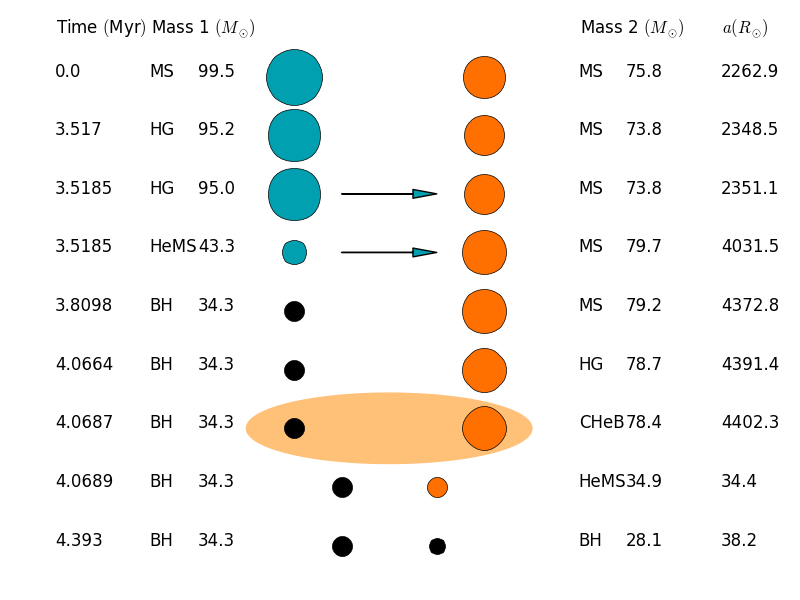
\includegraphics[width=0.9\textwidth]{COMPAS.png}
	\caption{\label{fig:COMPAS} A sketch of the possible evolutionary path of GW150914, following \citet{Stevenson:2017}.  The stars are born in a $Z=0.05 Z_\odot$ low-metallicity environment with an initial separation of $\sim 10$ AU.  The binary widens during non-conservative case B mass transfer from primary to secondary, but is hardened by two orders of magnitude as a result of dynamically unstable mass transfer from the expanding secondary onto the primary which has become a black hole.}
\end{figure}

Of course, this relatively simple picture holds many uncertainties: the rate of mass loss through winds, particularly during specific stellar evolutionary phases such as the luminous blue variable phase \citep{Mennekens:2014} and its dependence on metallicity; the efficiency of stable mass transfer efficiency; the response of a star to mass loss and the onset of a common envelope phase \citep{Pavlovskii:2017}; common-envelope survival and the amount of binary hardening associated with the envelope ejection; supernova fallback and natal kicks for black holes \citep[e.g.,][]{Repetto:2012,Mandel:2015kicks}; the possible contribution of double-core common envelopes when unstable mass transfer is initiated between two evolved stars; and the role of dynamically stable non-conservative mass transfer onto a lower-mass compact donor in achieving sufficient binary hardening  \citep{vandenHeuvel:2017,Neijssel:2018}.  We will discuss the possibilities of addressing some of these with future gravitational-wave observations in \autoref{prospect}.

\subsection{Abracadabra, thou shalt not expand: chemically homogeneous evolution}

What if we had a magic wand that could prevent stars from expanding?  Then a massive binary could start out at an orbital period of a couple days, close enough that if the stars made black holes in situ they would merge within the age of the Universe through the emission of gravitational waves, and remain there, without any mass transfer episodes including common envelope phases.  We may have gotten very lucky on this one: high-mass low-metallicity stars in close binaries may provide just such a magic wand for free.

Binary companions raise tides on each other, much like the Moon's tides on Earth.  If a binary is tight enough that each star fills a significant fraction of its Roche lobe, the tides get very large indeed, and the sloshing around as tidal bulges move over the star will dissipate a lot of energy -- unless, of course, the stars are tidally locked, and are always facing each other in the same way.  Thus, for close binaries, tidal locking becomes very efficient, and the rotation periods of the stars are synchronized to the orbital period of the binary.  By construction, this means that the stars are rotating at a few tens of percent of their break-up velocity.  Such rapidly rotating stars will develop significant temperature gradients between the poles and the equator, which may lead to efficient large-scale meridional circulation within the star \citep{Eddington:1925,Sweet:1950}.  \citet{EndalSofia:1978} and subsequent studies \citep[e.g.,][]{Heger:2000,MaederMeynet:2000,Yoon:2006} explored the internal shears and their impact on the mixing of chemical species within the star.  Although quantitative predictions differ, it appears that rapidly rotating massive stars may efficiently transport hydrogen into the core and helium out to the envelope until nearly all of the hydrogen in the star is fused into helium.  Then, at the end of the main sequence, the star behaves essentially as a Wolf-Rayet naked helium star, contracting rather than expanding.  There is no mass transfer, and as long as the metallicity is sufficiently low to avoid significant binary widening leading to the loss of co-rotating and chemically homogeneous evolution \citep{deMink:2009}, the binary can avoid mass transfer.  \citet{MandeldeMink:2016,deMinkMandel:2016,Marchant:2016} explored such binaries and concluded that they could present a viable channel for forming the most massive LIGO sources, such as GW150914, though not the lowest mass systems.

\subsection{The black hole matchmaking club: Dynamical formation in dense stellar environments}

The last possibility we will consider here is that the merging black holes may not have formed in the same binary at all.  Instead, they formed as a result of a collapse of massive stars independently, but were then introduced to each other by a matchmaker, or, rather, a whole array of matchmakers.  Suppose the two black holes formed in a dense stellar environment, such as a globular cluster.  Being the most massive objects in the cluster, they would naturally sink toward the cluster center as energy is equipartitioned through the cluster, a process known as mass segregation.  Once there, they will either form binaries through three-body interactions, or substitute into existing binaries: in a $2+1$ interaction, the lightest object is usually ejected in favor of the two heaviest objects forming a binary.  Subsequent interactions with the other objects in the cluster -- the matchmakers -- will gradually tighten the binary black hole, as the interloper is likely to leave with a slightly higher velocity than it came in with, reducing the energy of the binary.   If the density of objects is high enough to ensure a suitable rate of interactions, the binary will be hardened until it is compact enough to merge through gravitational-wave emission, provided it does not get kicked out of the cluster through a recoil kick from the last interaction (and even then, it may still go on to merge outside the cluster).  

The prospects for dynamical formed merging binary black holes in globular clusters have been developed through a series of analytical estimates and numerical experiments by \citet{Sigurdsson:1993,Kulkarni:1993,PZwart:2000,OLeary:2006,Banerjee:2010,Downing:2011,Morscher:2015,Mapelli:2016,Rodriguez:2016} and others.  \citet{OLeary:2008} and \citet{MillerLauburg:2008} have argued that dynamical formation could also take place in galactic nuclear with and without a massive black hole, respectively (but cf.~\citet{Tsang:2013} for the former).  \citet{Bartos:2016} and \citet{Stone:2016} have described the role that an accretion disk in an AGN could play in enhancing the rate of binary black hole mergers. Of course, dynamical formation need not be distinct from the evolution of an isolated binary system: for example, the inner binaries in hierarchical triple systems may evolve as isolated binaries, but then be brought together more efficiently through Lidov-Kozai oscillations \citep{Lidov:1962,Kozai:1962}; see, e.g., \citet{PeretsKratter:2012,Belczynski:2014VMS}.


\section{Merger rates and properties}\label{merge}

There are no known direct observations of binary black holes other than the sources observed by LIGO and Virgo through gravitational-wave emission (and a very speculative potential observation through microlensing \citep{Dong:2007}).  Therefore, beyond inference on the growing population of objects detected through gravitational waves, which we will return to in the next section, current knowledge of the merger rates and properties of binary black holes rests on modelling.  For the isolated binary evolution channel (\autoref{form}) this typically takes the form of forward modelling of large populations of stellar binaries distributed according to the observed initial mass and separation distributions in order to estimate the yield of merging binary black holes; this approach is known as population synthesis modelling.  Population synthesis techniques have also been applied to specific observed systems composed of a black hole and a Wolf-Rayet star, such as Cygnus X-1 \citep{Bulik:2008} and Cygnus X-3 \citep{CygnusX3:2012}, but whose future evolution is still uncertain.  The rate predictions from population synthesis models produced prior to 2010 are summarized by \citet{ratesdoc}.  Here, rather than delving into the details of binary evolution, we will attempt to estimate the relevant rates and expectations for the parameters of merging binary black holes, including their masses, spins, and environments.

In order to survive an evolutionary pathway such as the one depicted in \autoref{fig:COMPAS}, a binary must (i) have the right masses to form two black holes; (ii) have the right separation to avoid a premature merger, yet be close enough to interact; (iii) avoid disruption by supernova kicks; (iv) engage in and survive a common envelope phase; and (v) end up sufficiently compact at binary black hole formation to merge within the age of the Universe.  

The minimal initial stellar mass for forming a black hole is probably around 20 solar masses, so around $f_\textrm{primary} \approx 0.1\%$ of all stars drawn from the \cite{Kroupa:2002} initial mass function will form black holes. Although this can be shifted somewhat by binary interactions, for the purpose of this back-of-the-envelope calculation, we will use this approximation. Meanwhile, assuming that the mass ratio between the primary and the secondary is roughly uniformly distributed \citep{Sana:2012}, typically half the secondaries will fall into the mass range of interest, $f_\textrm{secondary} \approx 0.5$.  

The initial binary separations are observed distributed uniformly in the logarithm, $p(a) \propto 1/a$ \citep{Opik:1924}.  The first episode of mass transfer from the donor should typically be case B mass transfer (i.e., the donor should evolve beyond core hydrogen burning, but not yet beyond core helium burning); stars expand by several orders of magnitude during this phase, which means that the range of initial separations occupies a significant logarithmic fraction of the total initial range of separations, so $f_\textrm{init sep} \approx 0.5$.  We assume that black holes receive low natal kicks and do not lose significant amounts of mass, so that supernova do not significantly affect binary parameters, $f_\textrm{survive SN1} \approx f_\textrm{survive SN2} \approx 1$.  

The fraction of binaries that initiate and survive the common envelope phase during mass transfer from the secondary to the primary is perhaps the least certain.  Typically, it is easier to initiate a common envelope if the mass ratio of the donor to the accretor is greater, and when the donor begins mass transfer earlier in its post-main-sequence evolution.  The accreting black hole in this case may only have a third of the initial mass of the primary, with the rest lost with the envelope and through winds, while the secondary donor may have increased its mass during the first mass transfer phase; even so, unless the secondary was initially close to the primary in mass, the mass ratio is unlikely to exceed $3:1$, which is probably close to the threshold for initiating a common envelope phase.  At the same time, while an early onset of mass transfer means that the less evolved donor does not shrink as much in response to mass transfer (making mass transfer stable), it cannot have an envelope that is too tightly bound, otherwise the orbital energy is insufficient to eject it.  Together, these constraints reduce the fraction of successful common envelope initiations and ejections to $f_\textrm{CE} \approx 0.1$.  

Finally, there is the question of final separation at second black hole formation, as only systems with separations smaller than those in \autoref{fig:periapsis} will merge in the age of the Universe.  The final separation after the common envelope ejection is set by the binding energy of the envelope at the time when the secondary initiates unstable mass transfer, which in turn depends on the binary separation at that time.  Therefore, very crudely, the flat-in-the-log distribution of initial binary separations persists to the final binary separation.  Since the delay time between formation and merger $\tau_\textrm{GW} \propto a^4$ is a power law in the separation, the delay time distribution also follows a flat-in-the-log distribution $p(\tau) \propto 1/\tau$.  Among the binaries that survive a common envelope the closest will be those whose separations just barely encompass a Wolf-Rayet star, i.e., with separations of a few solar radii (and merger times of a few million years).  The logarithmic distribution ensures that tens of percent of binaries that survive a common envelope will merge in the age of the Universe, $f_\textrm{merge} \approx 0.2$.

Thus, we can write down a Drake equation for the probability that a stellar binary will end its life as a merging binary black hole:
\begin{eqnarray}
f_\textrm{BBH} &=& f_\textrm{primary} \times f_\textrm{secondary} \times f_\textrm{init sep} \times f_\textrm{survive SN1} \times f_\textrm{CE} \times f_\textrm{survive SN2} \times f_\textrm{merge} \nonumber \\
 & \sim & 0.001 \times 0.5 \times 0.5 \times 1 \times 0.1 \times 1 \times 0.4 = 5 \times 10^{-6}.
\end{eqnarray}
Merging binary black holes are rare outcomes indeed!  [Merging binary neutron stars are comparably rare: while stars with initial masses sufficient to form a neutron star, between roughly 8 and 20 solar masses, are more common than heavier stars necessary to form black holes, neutron star natal kicks and mass loss during a supernova are more likely to disrupt binaries, producing comparable yields.]

The star formation rate in the local Universe is $\sim 0.01 M_\odot$ Mpc$^{-3}$ yr$^{-1}$; for an average binary mass of $\sim M_\odot$, the yield $f_\textrm{BBH} \sim 5 \times 10^{-6}$ correspond to a binary black hole merger rate of $\sim 100$ Gpc$^{-3}$ yr$^{-1}$, or 10 per Myr for a Milky-Way equivalent galaxy with a space density of $0.01$ Mpc$^{-3}$.  Of course, the actual calculation of the binary merger rate requires significantly more care to account for the time-varying star formation history convolved with the time delay distribution.  The value of this back-of-the-envelope analysis is not so much in producing a merger rate that matches the rate inferred from gravitational-wave observations a posteriori, as in setting the stage for some of the predictions of the properties of merging binaries (see below) and the discussion of evolutionary uncertainties (see \autoref{prospect}).

The classical isolated binary evolution channel discussed in detail above can produce binary black holes with a broad range of masses matching all observations to date \citep[e.g.,][]{Stevenson:2017}, as well as GW170817 and the observed Galactic double neutron stars \citep[e.g.,][]{Kruckow:2018,VignaGomez:2018}.  In fact, contrary to mistaken lore, the high masses of the first observed black holes were not entirely surprising: such systems were predicted to arise in low-metallicity environments and make a significant contribution to the detected population because the more massive binaries emit more energy in gravitational waves \citep{Dominik:2014}.  Dynamical formation in globular clusters can also lead to a range of masses; it may have a stronger preference for more massive binaries as lighter black holes would be ejected by heavier ones in three-body interactions \citep{Rodriguez:2015}, but the mass distribution would be sensitive to natal kicks which may eject black holes at formation \citep{Zevin:2017}.  Chemically homogeneous evolution is only possible in more massive binaries, with total mass above $\sim 50 M_\odot$ \citep{MandeldeMink:2016,Marchant:2016}.

The masses of merging black hole binaries produced through the classical isolated binary evolution channel are likely to be on the equal side of $2:1$, because of the mass ratio constraints necessary to ensure stable mass transfer from the primary to the secondary and dynamically unstable reverse mass transfer, though mass ratios exceeding $2:1$ are more common at low metallicity \citep{Dominik:2012,Stevenson:2017}.  Dynamically formed binaries may also prefer comparable mass ratios because the heaviest black holes are most likely to merge, though more extreme mass ratios are also possible if the globular cluster contains a particularly heavy stellar-mass black hole or an intermediate-mass black hole \citep{Mandel:2008,Belczynski:2014VMS}.  On the other hand, chemically homogeneous evolution has a much stronger preference for equal masses \citep{MandeldeMink:2016}, with perhaps nearly equal mass black holes resulting from the evolution of systems that went through a contact phase \citep{Marchant:2016}.  

The spins of merging black holes may also carry imprints of their evolutionary history.  Isolated binaries are generally expected to have preferentially aligned spins after undergoing episodes of mass transfer and/or tidal coupling, although natal kicks and possible spin tilts during supernovae could lead to misalignment \citep[e.g.,][]{Farr:2011}.  Meanwhile, the spin directions are likely to be isotropically distributed for dynamically formed binaries \citep[e.g.,][]{Rodriguez:2016spin}.  

The spin magnitudes may also depend sensitively on the evolutionary history.  Although a massive star may contain a lot of angular momentum, far in excess of the maximum value allowed for a spinning black hole, the vast majority of that angular momentum will be contained in the outer layers of the star, and can therefore be readily lost through winds or through envelope stripping by a companion.  Therefore, black holes formed from stars that were rapidly spinning at some point in their evolution may still spin slowly unless stars are spun up through mass transfer or tides shortly before collapse \citep{Kushnir:2016,HotokezakaPiran:2017,Zaldarriaga:2017}.   This argument for slowly spinning black holes in compact binaries is potentially in conflict with the claimed observations of rapid spins in black-hole high mass X-ray binaries \citep{MillerMiller:2015}, but these may suffer from measurement systematics \citep[e.g.,][]{Kawano:2017}.  

Gravitational-wave spin measurements have so far only constrained the average spin component in the direction of the orbital angular momentum (so-called `effective spin'), which enters the phasing of gravitational waves at the 1.5 post-Newtonian order \citep{PoissonWill:1995}.  The low effective spins of the first four detected merging black holes allowed \citet{Farr:2017} to conclude that either the spin directions were isotropically distributed or the spin magnitudes were low.

The evolutionary history of merging black holes is also tied to their formation environments and delay times before merger.  
The yield of merging black holes per unit star forming mass is greatest at lowest metallicity, due largely to reduced wind-driven mass loss \citep[e.g.,][]{Belczynski:2010}; for the classical channel, delayed stellar expansion, which allows the stars to develop a larger helium core before engaging in mass transfer, further enhances this effect \citep[e.g.,][]{Stevenson:2017}.  Most of the low-metallicity star formation occurs in the early Universe, before gas is polluted with metal-rich products of stellar evolution, although there is a broad range of metallicities at all times \citep[e.g.,][]{LangerNorman:2006,TaylorKobayashi:2015}.  On the other hand, the delay time between star formation and merger in the classical formation channel peaks at shorter delay times with a $p(\tau) \propto 1/\tau$ decay.  A convolution of the metallicity-specific star formation history and the delay time distribution led \citet{Belczynski:2016} to conclude that, a posteriori, there was a bimodal probability distribution on the star formation history of GW150914, which either formed in the first $\sim$ Gyr after the Big Bang with a long subsequent delay to merger \citep{Dominik:2014}, or formed more recently in a low-metallicity region, such as a low-mass satellite galaxy.  

Finally, the eccentricity of merging black hole binaries may contain information about their past \citep{MandelOShaughnessy:2010}.  While isolated binaries are expected to merge on circular orbits as gravitational waves are very efficient at damping out eccentricity, dynamically formed systems may sometimes retain significant eccentricities if they are already very close at formation.  This may be possible either through two-body captures in Galactic nuclei \citep{OLeary:2008} \citet[but see][]{Tsang:2013}, or through close captures during three-body interactions \citep{Samsing:2014}.

\section{Prospects for gravitational-wave astronomy}\label{prospect}

Observed rates of binary black hole mergers indicate merger rates of around $\sim 10$ to $\sim 200$ Gpc$^{-3}$ yr$^{-1}$ \citep{GW150914:rates,GW170104}, which points to the prospect of tens of detections in the next observing run and hundred within the next three years, once the LIGO and Virgo instruments reach design sensitivity \citep{scenarios}.  This will yield enough information about both individually exciting events and population distributions to use gravitational-wave astronomy as a genuine tool for exploring stellar and binary evolution.  

Single events that can be individually informative include the discovery of a merging binary black hole with a component mass in the pair-instability supernova mass gap.  Models of pair instability supernovae suggest that no black holes with masses between $\sim 60 M_\odot$ (possibly reduced to $\sim 45 M_\odot$ by pulsational pair instability \citep{Woosley:2017}) and $\sim 130 M_\odot$ should form as a result of stellar collapse, with black holes on both sides of the mass gap possible \citep{Marchant:2016}.  Therefore, a discovery of a single object in this mass gap would point to either dynamical mergers that leave the merger remnant in the dense stellar environment to be reused, or to a theoretical failure in pair instability models.  Similarly, the discovery of a merger component with a mass between $\sim 2.3 M_\odot$ and $\sim 5 M_\odot$, in the range between the most massive known neutron stars and least massive black holes \citep{Ozel:2010,Farr:2011} would shed light on the supernova explosion models, specifically the amount of fallback that can occur before the explosion \citep{Fryer:2012}.

Other individually exciting events could include the first confirmed discovery of an intermediate mass black hole in the few-hundred solar-mass range, either as a merger of two such black holes \citep[e.g.,][]{Veitch:2015,Graff:2015} or as an intermediate-mass-ratio inspiral into such an object \citep[e.g.,][]{Haster:2015IMRI,Haster:2016}.  A source with a detectable in-band eccentricity would clearly signal a dynamical capture \citep{Breivik:2016}.  Meanwhile, a measurement of an effective spin value close to either 1 or $-1$ would point to rapid spins of both black holes.  A substantial positive effective spin coupled with high masses would point to the likelihood of chemically homogeneous formation \citep{Marchant:2016}, while a substantially negative effective spin measurement would indicate the absence of alignment, likely either through a spin tilt or dynamical formation.  

Population statistics will generally contain more information than individual events.  We can distinguish the approaches to inference on the observed populations into unmodeled or weakly modeled inference and inference that relies on accurate models. At the most basic end of weakly modeled inference is the (possibly non-parametric) reconstruction of the underlying distribution, such as the mass function of merging black holes \citep{Mandel:2010stat,BBH:O1} while accounting for measurement uncertainties and selection effects.  Similarly, the time delay between star formation and binary merger could be extracted by comparing the merger rate as a function of redshift against the star formation rate as a function of redshift \citep{Mandel:2016select}.

We can look for clustering of events by observed parameters in the hope of finding distinct clusters of systems corresponding to different subpopulations or evolutionary channels.  \citet{Mandel:2015} argued that $\sim 60$ observations would make it possible to cluster events by mass even after allowing for the significant measurement uncertainties inherent in gravitational-wave astronomy, and \citet{Mandel:2016cluster} demonstrated the feasibility of a particular clustering technique.  Meanwhile, \citet{Farr:2018} propose classifying binary black hole mergers by spin misalignment angle into aligned and isotropically distributed subpopulations.  It's worth noting that such clustering or classification schemes cannot hope to correctly assign individual events to a specific cluster, which is generally impossible given the significant measurement uncertainties \citep{Littenberg:2015}; instead, the goal is to measure the relative frequencies of events in different categories.

The next level of population-based inference relies on assuming that precise, possibly parametrized, subpopulation distributions are known to determine the ratios of different subpopulations (e.g., arising from different formation channels), typically using hierarchical modeling \citep[extreme deconvolution in the language of][]{Hogg:2010}.  \citet{Zevin:2017} found that the mass distribution alone could be used to determine the formation channel with $\sim 100$ observations, assuming trustworthy models of the mass distribution under different formation channels are available.  \citet{Vitale:2015,Stevenson:2017spin} carry out a similar investigation for spin-orbit misalignment angles; although these cannot be measured with the same accuracy as chirp masses, several hundred observations should again be sufficient to distinguish multiple formation channels through hierarchical modelling if the distributions under different channels are known \citep{Stevenson:2017spin}.   

Of course, there is a multitude of uncertain physics within a given model.  How much mass do stars lose in winds, and what is the precise impact of metallicity and rotation on stellar evolution \citep[e.g.,][]{Renzo:2017}?  What happens to the star's angular momentum during collapse, how much mass is ejected, and how much of an asymmetric kick does the star receive \citep[e.g.,][]{Mirabel:2016}? How conservative is mass transfer in binaries and how much angular momentum is carried away by the mass lost from the binary during non-conservative mass transfer \citep[e.g.,][]{vandenHeuvel:2017}?  What are the conditions for the onset of a common-envelope phase and the common envelope ejection, and how does the binary change in the process \citep[e.g.,][]{Ivanova:2013}?   How do dynamical interactions affect binary evolution?  And, in turn, how do massive stellar binaries and their compact remnants feed back into astrophysics and cosmology on all scales?

One approach to addressing these big questions is to use the framework of population synthesis, which makes it possible to parametrize the uncertain physics and predict the expected source rates and distributions under different models.  Early  efforts relied on a discrete set of a few models in the parameter space of population synthesis assumptions \citep{Dominik:2012,Stevenson:2015}.  Even with the low computational cost of population synthesis, it is not feasible to explore more than a few tens to a few hundred models, which is not sufficient to explore the full parameter space or consider the correlations between model parameters.  However, recent successes in building accurate and computationally efficient emulators over the model parameter space \citep{Barrett:2017} suggest that a full exploration of this space will soon be possible. \citet{Barrett:2017FIM} applied Fisher information matrix techniques to the space of model parameters and found that parameters such as mass loss rates during the Wolf-Rayet phase and common envelope energetics can be measured to the level of a few percent with a thousand detections. 

More observational data sets will further aid in interpreting gravitational-wave observations.  Future missions raise the prospect of observing evolution of populations of merging binaries -- or event individual systems -- across a broad band of gravitational-wave frequencies, from the millihertz \citep[e.g.,][]{Sesana:2016} through the decihertz \citep{Mandel:2017} and hertz \citep{ET:2012} to the LIGO/Virgo band.  Although electromagnetic transients are not broadly expected to be associated with binary black hole mergers \citep[e.g.,][]{Lyutikov:2016}, any such observations would indicate the persistence of material around the merging binary \citep[e.g.,][]{deMinkKing:2017}.  %\todo{More details -- brief summary of Lorentz center workshop?}

The most useful additional constraints, however, are likely to come from comparing other data sets with gravitational-wave observations and demanding that any evolutionary model must self-consistently explain all of the available data: gravitational-wave observations, X-ray binaries, Galactic neutron stars, gamma ray bursts, supernovae, luminous red novae, etc.   Incorporating these constraints will make it possible to resolve these degeneracies and build a concordance model of massive binary evolution.  %\todo{Other possible gravitational-wave sources? More details / references on XRBs, LRN, etc.?}

The future of gravitational-wave astronomy holds the prospect of addressing the inverse problem of massive binary evolution: inferring the formation channels and their physics from observations of the merging compact-object binary population.  Like a paleontologist who uses her knowledge of anatomy to determine the appearance, eating habits, and even behaviour of extinct dinosaurs from their skeletal remnants, we can now use merging neutron stars and black holes ? remnants of massive stars ? to probe the behaviour of those stars, and particularly their evolution in binaries \citep{MandelFarmer:2017}.   With the data to come and the theoretical developments underway, this future is brightly chirping indeed!


\begin{acknowledgements}
IM thanks all of the people who have guided him to understand stellar and binary evolution, foremost among them Selma de Mink.   The students who contributed to building COMPAS (Simon Stevenson, Alejandro Vigna G\'{o}mez, Coenraad Neijssel -- who deserves special thanks for assistance with figures \ref{fig:BHremnant} and \ref{fig:Rmax}, Jim Barrett, Sebastian Gaebel) and external collaborators (including Stephen Justham and Philipp Podsiadlowski) deserve particular thanks.  Thanks also to Cole Miller, Vicky Kalogera, and Will Farr for stimulating discussions spanning many years.
\end{acknowledgements}

\bibliographystyle{hapj}
\bibliography{Mandel}

\end{document}

